\documentclass{article}

\usepackage[T1]{fontenc}
\usepackage[utf8]{inputenc}
\usepackage{graphicx}
\usepackage{parskip}
\usepackage{comment}
\usepackage{amsmath}
\usepackage{amssymb}
\usepackage[a4paper, margin=2cm]{geometry}
\usepackage{ulem}
\usepackage{listings}
\usepackage{xcolor}
\usepackage{bm}
\usepackage{tabularx}

\graphicspath{{ ./images/ }}
\renewcommand{\familydefault}{\sfdefault}
\renewcommand{\ULdepth}{1.5pt}

\makeatletter
\newcommand*{\saved@uline}{}
\let\saved@uline\uline
\newcommand*{\mathuline}{%
  \mathpalette{\math@uline\saved@uline}%
}
\newcommand*{\math@uline}[3]{%
  \mbox{#1{$#2#3\m@th$}}%
}
\renewcommand*{\uline}{%
  \relax  
  \ifmmode \expandafter\mathuline
  \else \expandafter\saved@uline \fi
}
\newcommand*{\vc}[1]{\ensuremath{\boldsymbol{{#1}}}}
\newcommand*{\mt}[1]{\ensuremath{\boldsymbol{\mathbf{#1}}}
}
\newcommand*{\ndist}[2]{\ensuremath{\sim \mathcal{N}(#1, #2)}}
\newcommand*{\Ndist}[3]{\ensuremath{\sim \mathcal{N}(#1; #2, #3)}}
\newcommand*{\ndistfn}[3]{\ensuremath{\frac{1}{#3\sqrt{2\pi}}\exp{ \left[- \frac{1}{2} \left(\frac{#1 - #2}{#3}\right)^2 \right]}}}
\newcommand*{\expect}[1]{\ensuremath{\mathop{{}\mathbf{E}}\left(#1\right)}}
\newcommand*{\qt}[1]{`#1'}
\newcommand{\vvc}[1]{\begin{bmatrix}#1\end{bmatrix}}
\newcommand*{\dd}[2]{\frac{\partial{#1}}{\partial{#2}}}
\makeatother

\title{Least Squares Regression Report: \\ An Unknown Signal}
\author{Taharka Okai}
\date{April 2021}

\begin{document}
\maketitle

\section{Linear regression}

\label{sec:Linear regression}

Consider the case where a pair $(x, y)$ related by $f$ where $y = f(x)$ can be estimated by a \qt{guess} function $\hat y = \hat f(x)$. The likelihood of the output given the estimate, assuming that the likelihood is described by a normal distribution, yields the following:

\[
  P\left(y |\hat y \right) = \ndistfn{ y}{\hat y}{\sigma}
\]

However nothing is known about the value of $\hat y$ as the function describing the estimate is still unknown. It is possible to ``design'' a function by expressing $\hat f(x)$ as a matrix product between a vector containing functions of $x$, or features and different scaling factors for each feature, or weights. Below is an example:

\[
  \text{Take }\hat f(x) = 2x + 3.\text{ Then }\hat f(x) = {\vc x}^T \vc w\text{ where } \vc x = \vvc{ 1 & x }\text{ and } \vc w = \vvc{ 2 \\ 3}
\]

Note that the above can be extended where the input space is a vector. Using this structure, the likelihood can be rewritten in terms of the feature and weight vectors. The above only considers a case where a single estimator for $y$ is considered, but when working with vectors, the product of all likelihoods for each dimension in $y$ represents the overall likelihood given $\hat {\vc y}$.

Using log values of the likelihood not only makes the calculation of probabilities more stable during computation - as the probabilities tend to be small - but also reduces the product of the likelihoods in the equation to a sum (because $\log \prod_i x_i = \sum_i \log x_i $), making the differentiation step easier to calculate.

\[
  \def\yhat{{\vc x_i}^T {\vc w_i}}
  \begin{aligned}
                       &
                       & P\left( \vc y_i | {\vc x_i}, \vc w_i \right)
                       & = \ndistfn{\vc y_i}{\yhat}{\sigma}
    \\
    \mathcal{L}(\vc w) & =
                       & \log \left( \prod_i  P\left( \vc y_i | {\vc x_i}\right), \vc w_i \right)
                       & = -\frac{1}{2} \sum_i \left( \log{2\pi\sigma^2} + \frac{1}{\sigma^2}\left(\vc y_i-\sum_j{\mt X_{ij}\vc w_j}\right)^2 \right)
  \end{aligned}
\]

Using the equation above it is possible to maximise the likelihood using the single free parameter in this equation, $\vc w$. Finding the solution to $\dd{\mathcal{L}\left({\vc w}\right)}{\vc w}=\vc{0}$ produces $\vc {\hat w}$, the value of the weight vector that maximises $P(\vc y|\mt X, \vc w)$:

\[
  \begin{aligned}
    \dd{\mathcal{L}\left({\vc w_k}\right)}{\vc w_k}
      & = -\frac{2}{2\sigma^2}\sum_i\left(
    \left(\dd{\vc y_i}{\vc w_k}+\sum_j{\dd{\vc w_j}{\vc w_k}\mt X_{ij}}\right)
    \cdot\left(y_i - \sum_j{\mt X_{ij}\vc w_j}\right)
    \right)
    \\
    0 & = - \frac{1}{\sigma^2}\sum_i\left(0 + \mt X_{ik}\right)\cdot(y_i - \sum_j{\mt X_{ij}\vc w_j}) = \sum_i{\mt X_{ik}\left(y_i - \sum_j {\mt X_{ij} \vc w_j} \right)}
  \end{aligned}
\]

\[
  \scriptstyle{\text{Since }\vc w_j \text{ is independent of } \vc w_k \text{ when } j = k, \dd{\vc w_j}{\vc w_k}=1, \text{ and }0\text{ otherwise }}
\]

Thus remains:

\[
  \begin{aligned}
    {\mt X}^T{\mt X}{\vc y}-{\mt X}^T{\mt X}{\vc {\hat w}} & ={\vc 0}                                            \\
    \vc {\hat w}                                           & = \left({\mt X}^T {\mt X}\right)^{-1}{\mt X}^T\vc y
  \end{aligned}
\]

To finally calculate the value of $\hat y$ and estimate $y$, simply substitute the maximising weight vector into the equation for $\hat f(x)$.

\[
  \vc y \approx \vc {\hat y} = {\vc x}^T \hat w
\]

\section{Method}
\label{sec:Method}

\subsection{Nomenclature}

The features describing the general characteristic of a function's properties, like the shape of its graph, will be referred to as the \qt{class} of the function.

The function on $x$ with the highest coefficient or exponent of fitted function's class will be referred to as the \qt{order}, where $\sin(3x)$ is of greater order than $\sin(x)$. This comparison does not apply between function classes, however.


\subsection{Observations}

Firstly the files provided were parsed to retrieve data and assigned to input and output vectors, extended as described in the previous section. Then functions were chosen that would supposedly fit into the three given types, linear, polynomial or unknown.

\begin{table}[h!]
  \begin{center}
    \begin{tabular}{
        | m{5em} | m{20em} | m{10em} |
      }
      \hline
      Function    & Form                                                    & $\vc {\hat w}$                                       \\
      \hline\hline
      Linear      & $a+bx$                                                  & $\vvc{a        & b}^T$                               \\ \hline
      Polynomial  & $a+bx+cx^2+dx^3+\cdots$                                 & $\vvc{a        & b     & c & d          & \cdots}^T$ \\ \hline
      Exponential & $a+e^{bx}$                                              & $\vvc{a        & b}^T$                               \\ \hline
      Sinusoidal  & $a + \sin(bx) + \cos(bx) + \sin(cx) + \cos(cx)+\cdots $ & $\vvc{a        & b     & c & \cdots}^T$              \\ \hline
    \end{tabular}
  \end{center}
  \caption{Functions to fit for $\vc {\hat w}; \vc{\hat y}$}
  \label{tab:fnclasses}
\end{table}

A large set of Python lists were generated containing function objects with the specified parameters, for example calling \texttt{Model.\-polynomial(3)} would result in a feature vector matching the polynomial of order 3. A \qt{training set} would be a hard coded subset of the available functions mentioned in Table \ref{tab:fnclasses}, for example, \{ linear, polynomial(2), polynomial(3), exponential, sinusoidal(2) \}. Additionally, upon controlled test runs, the maximum order for the sinusoidal and polynomial functions were reduced to 3 and 5 respectively, as those models were seldom chosen as suitable models for the provided dataset.

An observation that the exponential model was not chosen once by the algorithm indicates one of three possible things - either the exponential model was a poor choice for fitting these specific functions, the model was not extensive enough (i.e. not enough terms) or the model was not described correctly (i.e. $a + e^{bx}$ is the wrong form.)

\subsection{Determining function class}

Running these tests resulted in the plots shown in Figure \pageref{fig:unaccounted}. The algorithm progressively finds the model with the least cross validation error for each segment, meaning that the model with the least residuals gets chosen. This aims to produce accurate looking plots. However this does not yet account for possible overfitting, as part of the assignment is to ensure that the order for each class of function is consistent between files.

\begin{figure}[!hbt]
  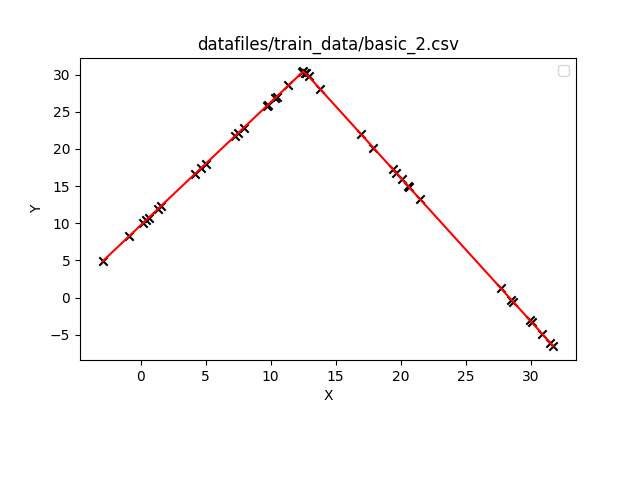
\includegraphics[scale=0.34]{./images/basic_2}
  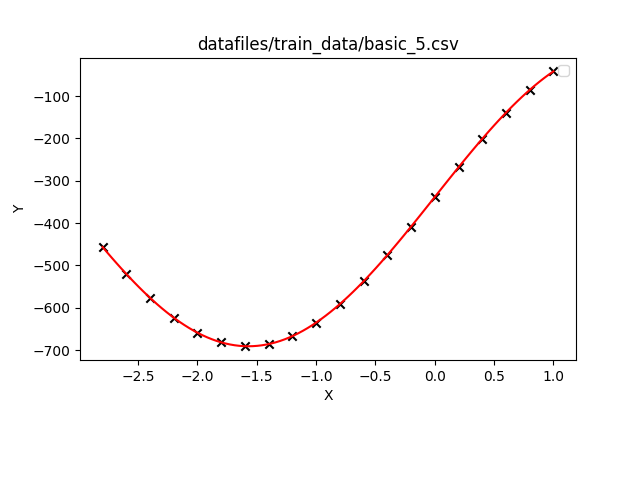
\includegraphics[scale=0.34]{./images/basic_5}
  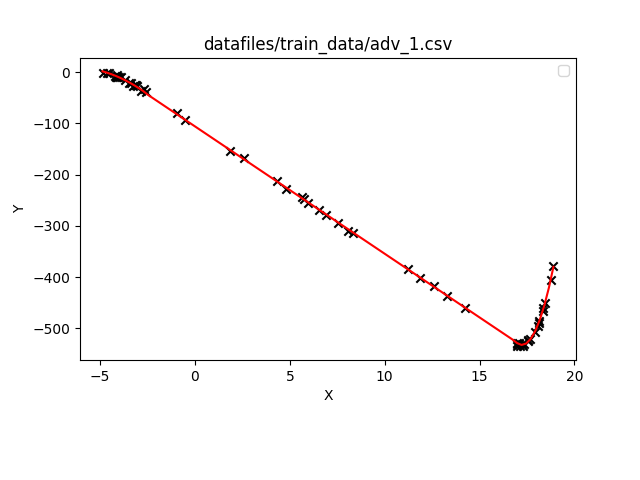
\includegraphics[scale=0.34]{./images/adv_1}
  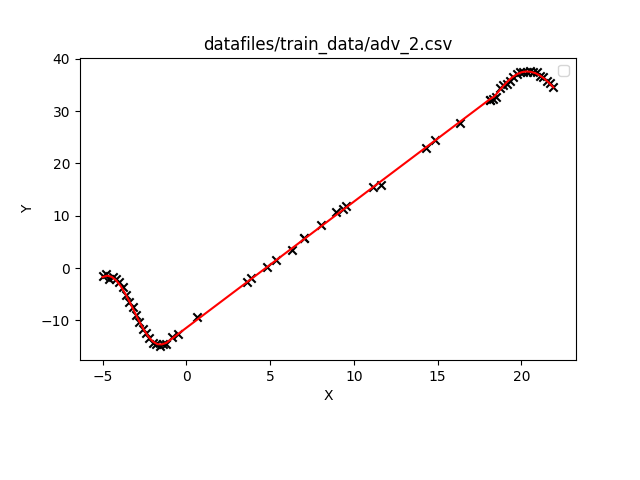
\includegraphics[scale=0.34]{./images/adv_2}
  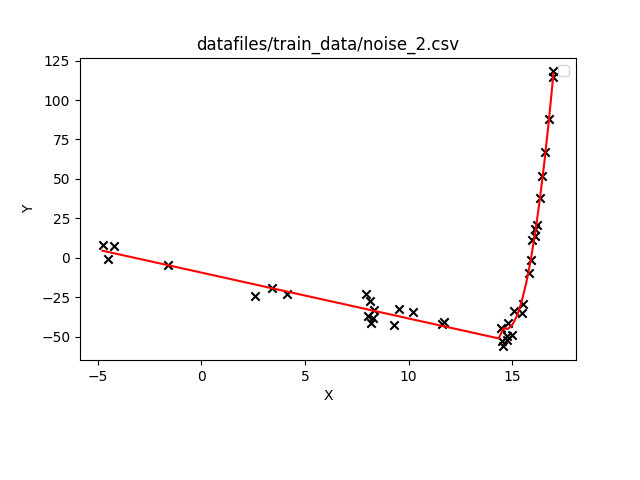
\includegraphics[scale=0.34]{./images/noise_2}
  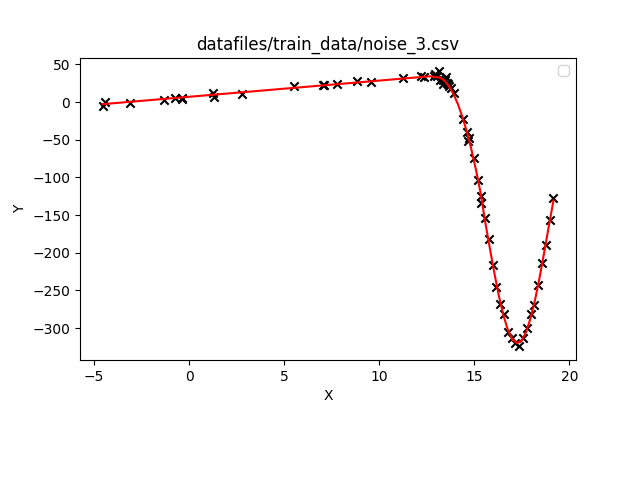
\includegraphics[scale=0.34]{./images/noise_3}
  \caption{Some unaccounted-for fitted model results (no class determination)}
  \label{fig:unaccounted}
\end{figure}

\subsection{Determining function order}

The strategy for determining the common unknown and polynomial classes over each file was to be that for each segment with a specific set of class (i.e. polynomial, sinusoidal), the program would determine whether the order was disparate between files. For example if one segment was fitted to a quadratic and another to a cubic - the same class but different order. In this specific cases, the disparate orders would be collected in a list and the algorithm run again for these segments, except instead of minimising error across function classes, the program would attempt to minimise error over order, to choose the best order that minimises error over all files considered. The results of this are shown in Table \ref{tab:order}. In this instance, the functions chosen would be the order 4 polynomial and the order 2 sinusoid.

\begin{table}[!hbt]
  \begin{center}
    \begin{tabular}{| m{10em} | m{9em} |}
      \hline
      Function class        & Sum-squared Error \\ \hline
      Polynomial order 3    & 3514.69           \\ \hline
      Polynomial order 4    & 3283.77           \\ \hline
      Sinusoid \qt{order} 1 & 1199.00           \\ \hline
      Sinusoid \qt{order} 2 & 1124.00           \\ \hline
    \end{tabular}
  \end{center}
  \caption{The Sum-squared error over segments of multiple order classes}
  \label{tab:order}
\end{table}

\section{Shortcomings}

A possible caveat in the algorithms cross validation process is that a systematic approach to the selection of 50\% of the points, a number chosen arbitrarily, was carried out. This may have steepened the correlation of the function between the points in the training set and the points in the validation set. The attempt to counterbalance this was to alternate between the cross-validation and training sets and select the function with the least cross validation error. 

While this did create stability in the output (because the set of points removed from the training set per iteration was the same), this is a non-standard technique and may cause some biases in the fitting. For example, the fact that the input space is not uniformly distributed (i.e. the difference between adjacent points on the x-axis can vary wildly). Perhaps too many points were removed from the validation set for the results to be close to the true answer. 

Observable oversights of the approach to determining the order of the function include the lack of evidence supporting the claim that this is a suitable way to mitigate overfitting. In hindsight, a reduced sum squared error at a higher order may be indicative of overfitting, so this method is by no means entirely reliable. Due to programming bugs and time restraints, graphs for the selected order for the functions were unfortunately not included in this document.

\end{document}